% Created 2024-08-30 Fri 17:18
% Intended LaTeX compiler: pdflatex
\documentclass[letterpaper, 11pt]{article}
\usepackage[utf8]{inputenc}
\usepackage[T1]{fontenc}
\usepackage{graphicx}
\usepackage{longtable}
\usepackage{wrapfig}
\usepackage{rotating}
\usepackage[normalem]{ulem}
\usepackage{amsmath}
\usepackage{amssymb}
\usepackage{capt-of}
\usepackage{hyperref}
\usepackage{minted}
\usepackage{xcolor}
\usepackage{hyperref}
\usepackage{tocloft}
\usepackage[margin=1in]{geometry}
\usepackage{fancyhdr}
\usepackage{fancyheadings}
\usepackage{titlepic}
\usepackage{pdfpages}
\usepackage[T1]{fontenc}
\usepackage{helvet}
\usepackage{fontawesome}
\usepackage[colorlinks=true, urlcolor=blue, linkcolor=blue]{hyperref}
\usepackage{graphicx}
\usepackage[mmddyyyy]{datetime}
\setlength{\parskip}{2mm}
\setlength{\parindent}{0mm}
\usepackage{setspace}
\usepackage{wrapfig}
\hypersetup{breaklinks=true}
\usepackage{verbatim}
\usepackage{fvextra}
\usepackage{float}
\usepackage{lipsum}
\author{Hilduara Abreu}
\date{\today}
\title{PS192 Handbook}
\hypersetup{
 pdfauthor={Hilduara Abreu},
 pdftitle={PS192 Handbook},
 pdfkeywords={},
 pdfsubject={},
 pdfcreator={Emacs 29.4 (Org mode 9.6.15)}, 
 pdflang={English}}
\begin{document}

\maketitle
\tableofcontents


\section{Cover Page}
\label{sec:orgb27ec8f}
\thispagestyle{empty}
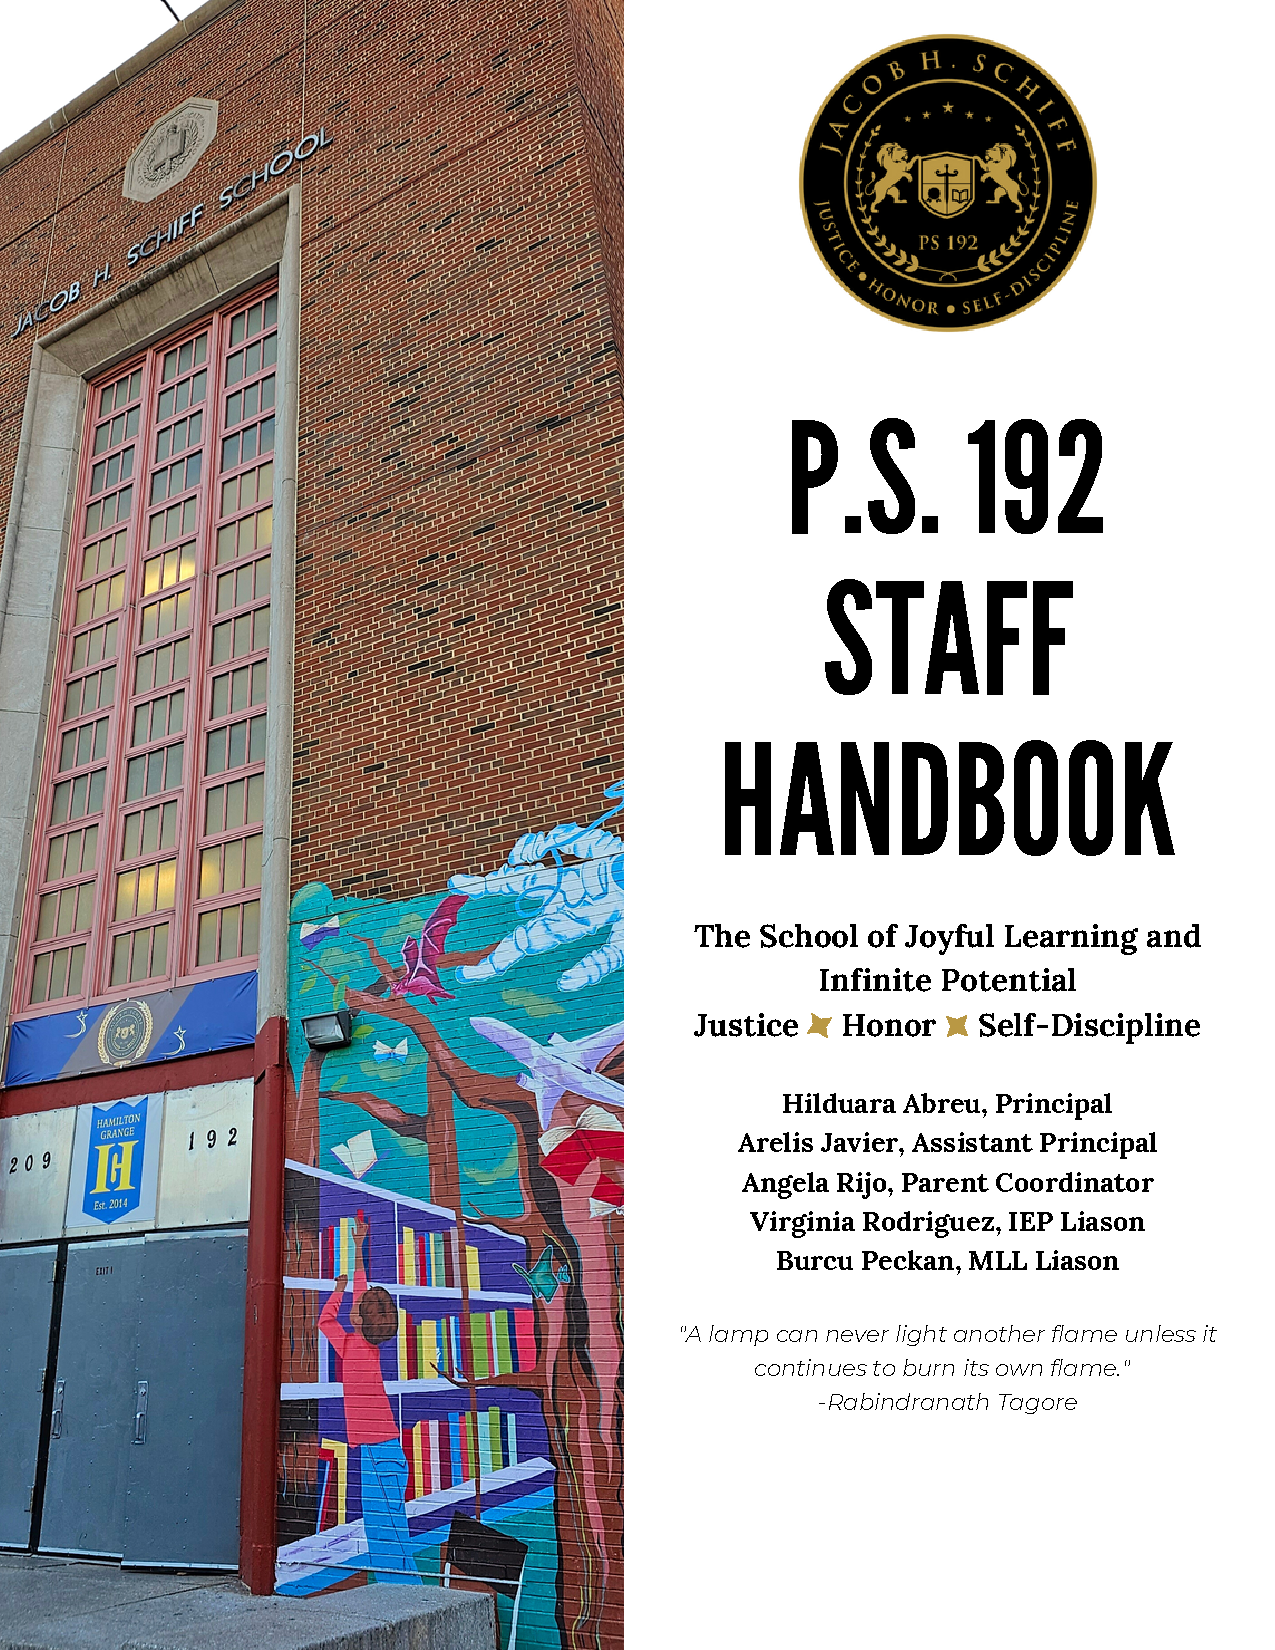
\includepdf[pages=1,fitpaper]{handbook_front.pdf}

\section{Header and Footer}
\label{sec:org86e64d1}
\pagenumbering{\fancyhf{}}
\pagestyle{headings}
\pagenumbering{arabic}
\fancyhead[L]{\textit{\rightmark}}
\fancyhead[R]{\thepage}
\fancyfoot[C]{The School of Joyful Learning!}
\pagestyle{fancy}
\renewcommand{\footrulewidth}{1px}

\section{Table of Content}
\label{sec:orgebb1470}
\setcounter{tocdepth}{2}
\tableofcontents

\section{Message from the Principal}
\label{sec:orgd41795e}
Hilduara Abreu

Dear Staff:

Welcome to the 2023-2024 edition of the PS 192: Jacob H. Schiff Faculty and Staff Handbook. It is the responsibility of each staff member to be fully acquainted with the information contained herein. This handbook is a living document and it will be updated, as necessary, throughout the year. It is meant to provide information and procedures that are important for the smooth operation of our PS 360 community. This handbook is a guide for ALL STAFF MEMBERS about the daily operation of our school. Please familiarize yourselves with your individual and school-wide responsibilities. Please do not hesitate to ask questions or get further clarification regarding any policy or procedure.

I encourage you to begin by thoroughly acquainting or re-acquainting yourself with our school’s philosophy, mission, objectives, and core principles, as outlined in the School Overview. Key elements of this vision are elaborated upon throughout the handbook, along with important information about structures and policies that support our school mission and ensure the safety and success of all members of our school community.

During the upcoming school year, we will continue to strengthen and deepen our work in relation to NYCDOE and District 6 priorities, as reflected in our School Problem of Practice, priorities, and CEP Goals. These areas will be central to our work as a Professional Learning Community and will be further addressed in Professional Learning sessions and Professional Planning Teams, as well as in administrative memos and guidelines, many of which can be accessed in Appendix B of this handbook.

I look forward to our continued collaboration in the year ahead.

Respectfully yours,


\includegraphics[width=0.2\textwidth]{hil_signature}

\textbf{Hilduara Abreu, Principal}

\textbf{\textbf{The School of Joyful Learning!}}

\href{https://www.ps192.org}{www.ps192.org}

\pagebreak

\section{Acknowledgment of Receipt and Review}
\label{sec:orge7244bd}
\subsection{Date: \href{https://www.ps192.org}{September, 2023}**}
\label{sec:org7d6b055}

\textbf{\textbf{Subject: Faculty and Staff Handbook Acknowledgment of Receipt and Review}}

I,:\line(1,0)\{150\}(staff member name), hereby acknowledge that I have read and understand the contents of the Faculty and Staff Handbook, including Appendix A: Chancellor’s Regulations, as well as the PS 192 Family Handbook and Citywide Behavioral Expectations to Support Student Learning. I understand that I am also responsible for following the directives included in Appendix B: Administrative Memos, as well as subsequent administrative directives that may be issued during the year. I will adhere to the policies and procedures set forth in the PS 192 Faculty and Staff Handbooks, the Chancellor’s Regulations, and all Administrative Memos.

\vspace{3mm}
\faSquareO \hspace{1em} I have reviewed the The P.S. 192 Staff Handbook

\begin{center}
\noindent\begin{tabular}{ll}
\makebox[2.5in]{\hrulefill} & \makebox[2.5in]{\hrulefill}\\
Teacher's Signature & Date\\[8ex]% adds space between the two sets of signatures
\makebox[2.5in]{\hrulefill} & \makebox[2.5in]{\hrulefill}\\
Assistant Principal & Date\\[8ex]% adds space between the two sets of signatures
\end{tabular}
\end{center}

\begin{center}
\begin{figure}
\centering

\includegraphics[width=50mm,scale=0.5]{himher1}
  \label{fig:school logo}
\end{figure}
\end{center}

\newpage

\section{School Overview}
\label{sec:org034816e}
PS 192 Jacob H. Schiff (06M192) is a District 6 public school that serves children from diverse cultural, linguistic, and socio-economic backgrounds. The success of our students and community relies on our continuous elementary learning experience, dedication, knowledge, teamwork, and collaboration. Our school provides a well-balanced looping education that will be a bridge to opportunity and success. To meet our students’ needs, our programs this year will focus on a standards-based rigorous curriculum that motivates and inspires students to make connections between our school and their future. We focus on students’ strengths and build self-esteem through authentic and rigorous achievement. We recognize that students can and will value their educational experience because they see, feel, and understand the connection to their personal lives. Preparing our students for College and Career Readiness continues to be at the foundation of all our work.

\begin{wrapfigure}{R}{0.4\textwidth}
\centering
\includegraphics[width=0.6\textwidth]{logohim.jpg}
\end{wrapfigure}

\subsection{Core Values}
\label{sec:org0c4ccaf}
At P.S. 192, we uphold a set of core values that serve as the foundation of our educational community. These values, rooted in justice, honor, and self-discipline principles, guide our actions, decisions, and interactions, creating a culture of integrity and excellence.

\begin{itemize}
\item Justice: We are committed to fairness and equality for all members of our school community. We believe in the equitable treatment of every individual, irrespective of their background, ensuring that each student has the opportunity to thrive academically and personally. Our commitment to justice fosters an inclusive and supportive environment where every voice is heard, valued, and respected.
\item Honor: Integrity is the cornerstone of our educational philosophy. We encourage our students to act with honesty and integrity in all aspects of their lives. Upholding honor means taking responsibility for one's actions, demonstrating ethical behavior, and consistently adhering to a code of moral values. We believe that integrity is the pathway to personal growth and societal betterment.
\item Self-Discipline: We recognize the importance of self-control and self-mastery in achieving success. At P.S. 192, we instill in our students the value of self-discipline as an essential skill for achieving their goals and aspirations. Through self-discipline, our students learn to set priorities, manage their time effectively, and overcome challenges, ultimately becoming responsible and accountable individuals.
\end{itemize}

These core values of justice, honor, and self-discipline guide us in pursuing academic excellence and character development. By embracing these principles, we empower our students to become responsible citizens, compassionate leaders, and lifelong learners who contribute positively to our global community. At P.S. 192, we are dedicated to nurturing academic achievements and the values and qualities that will shape our students into ethical, compassionate, and successful individuals.

\subsection{Vision}
\label{sec:org6f22c6a}
To ensure all students acquire the essential knowledge and skills they need to become independent thinkers, active participants, and contributors in their roles as students and as members of society.

\subsection{Mission}
\label{sec:orgfb3df4d}
To provide a welcoming, safe, resourceful, and nurturing environment that supports our school community's academic and social-emotional development where children are respected and engaged in challenging curricula that motivate them to realize their potential as active, lifelong learners. Through our guiding core values of Justice, Honor, and Self-discipline, we aspire to promote perseverance, love, empathy, and respect for oneself and others.

\subsection{School Motto}
\label{sec:org5a14ad7}
"Good, better, best. Never let it rest until your good is better, and your better is best."  -St. Jerome

\section{Educational Philosophy}
\label{sec:orge474d69}
We believe that relationships, with oneself and with others, form the basis of learning and teaching. These relationships extend beyond the classroom to include children’s families and the multiple communities of which they are a part. By building meaningful relationships among school, home, and the wider community, we seek to instill in each child an integral sense of continuity and connection that will support his or her growth in its many dimensions.

Learning is a natural human process inherent to all children, transcending cultural, socio-economic, and learning differences. Children’s innate interests and capabilities are essential to the learning process. A stimulating and engaging environment can awaken a sense of wonder and intellectual curiosity that must be carefully guided and fed. Students learn best when teachers draw upon their existing understandings and help them build new understandings based on increasingly complex knowledge. To this end, our school integrates child-centered pedagogies with rigorous, content-rich instruction in response to ongoing assessment of individual student needs.

\subsection{Core Principles}
\label{sec:org541d0ed}
The vision for Jacob H. Schiff is guided by the following core principles:
\begin{itemize}
\item An effective learning environment places meaningful relationships—among teachers, students, families, and other community members—at its center.
\item Small learning communities, in which adults and children know each other well, provide rich opportunities for personal, social, and intellectual development.
\item Families play an essential role in their children’s education and should therefore be invited to participate in multiple aspects of school life.
\item A community-based school must be accessible, accountable, and responsive to all families, regardless of their linguistic, cultural, socioeconomic, or educational backgrounds.
\item Children benefit from a coherent academic program that encompasses Pre-Kindergarten to Grade 5.
\item All children have gifts and talents, which can be effectively fostered in heterogeneous classrooms in which adults hold high expectations for every student.
\item Children learn through active engagement and exploration, and by constructing understandings based on their own experiences and observations.
\item A language-rich environment, accessible to children of diverse backgrounds, provides the foundation for achievement in all academic disciplines and areas of life.
\item A well-rounded education provides academic rigor as well as opportunities for self-expression, artistic creation, and personal reflection.
\item Engagement in multicultural, multilingual learning environments will prepare children to participate fully in our diverse society.
\item Education should include not only the mastery of information and skills but also the development of critical thinking abilities and ethical awareness.
\end{itemize}


\includegraphics[width=1\textwidth]{positivity.pdf}

\subsection{Commitment to Achievement}
\label{sec:org6942a49}
In our commitment to delivering a rigorous, inclusive, and family-centered educational experience for the children of our community, PS 192 will:
\begin{itemize}
\item Uphold our identity as a dedicated learning community, earnestly striving to intimately understand each student and their family.
\item Cultivate an intellectually stimulating and captivating learning environment that prioritizes relationships as the primary conduit of both learning and teaching.
\item Assure that our students consistently attain and surpass academic benchmarks across all subject areas.
\item Incorporate family involvement and feedback at various levels of school administration.
\item Instill in every student elevated expectations for their own capabilities, reinforced by unwavering belief in their demonstrated aptitudes.
\item Conduct methodical evaluations of student learning assessments with the aim of scrutinizing data for patterns of misunderstandings and devising solutions to enhance student achievement.
\end{itemize}

\subsection{Commitment to Parental Engagement}
\label{sec:orgec00450}
\begin{wrapfigure}{L}{0.4\textwidth}

\includegraphics[width=0.5\textwidth]{logoher.jpg}
\end{wrapfigure}

Research consistently confirms that meaningful family engagement plays a pivotal role in the academic success of children. In light of this, Jacob H. Schiff holds family engagement and authentic home-school partnerships at the core of its mission.

At Jacob H. Schiff, we actively promote meaningful family engagement through regular opportunities for family involvement in classroom activities and school events. Our program design ensures that such involvement aligns with both the school's mission and the educational objectives set by our teachers and staff. Parents and other family members are encouraged to provide various forms of support, which may include preparing classroom materials, delivering curriculum-related presentations about their family experiences or cultural backgrounds, or sharing their expertise in areas such as music, dance, storytelling, science, or technology. Through these collaborative efforts, teachers and family members can establish mutual respect as valued partners in the education of all PS 192 students.

The relationship between the school and families is central to our mission. Consequently, we aspire to foster an active partnership that leverages the unique resources each student brings from their home environment. When families are deeply engaged in their children's learning and children witness their parents' dedication to their education, a vital connection is forged between the home and the school. By cultivating a cooperative partnership with each student's family, our goal is to emphasize the role of families as the ultimate stakeholders in the school and acknowledge their responsibility in the comprehensive education of each child.

As part of our commitment to transparent communication, each grade group is expected to send newsletters to families via grade-level Google groups at least twice a month. These newsletters will provide updates on curriculum developments within the classroom, upcoming field trips, suggestions for family outings and recommended books to enhance your understanding of your child's educational journey within our school.

\begin{figure}[H]
  \centering
  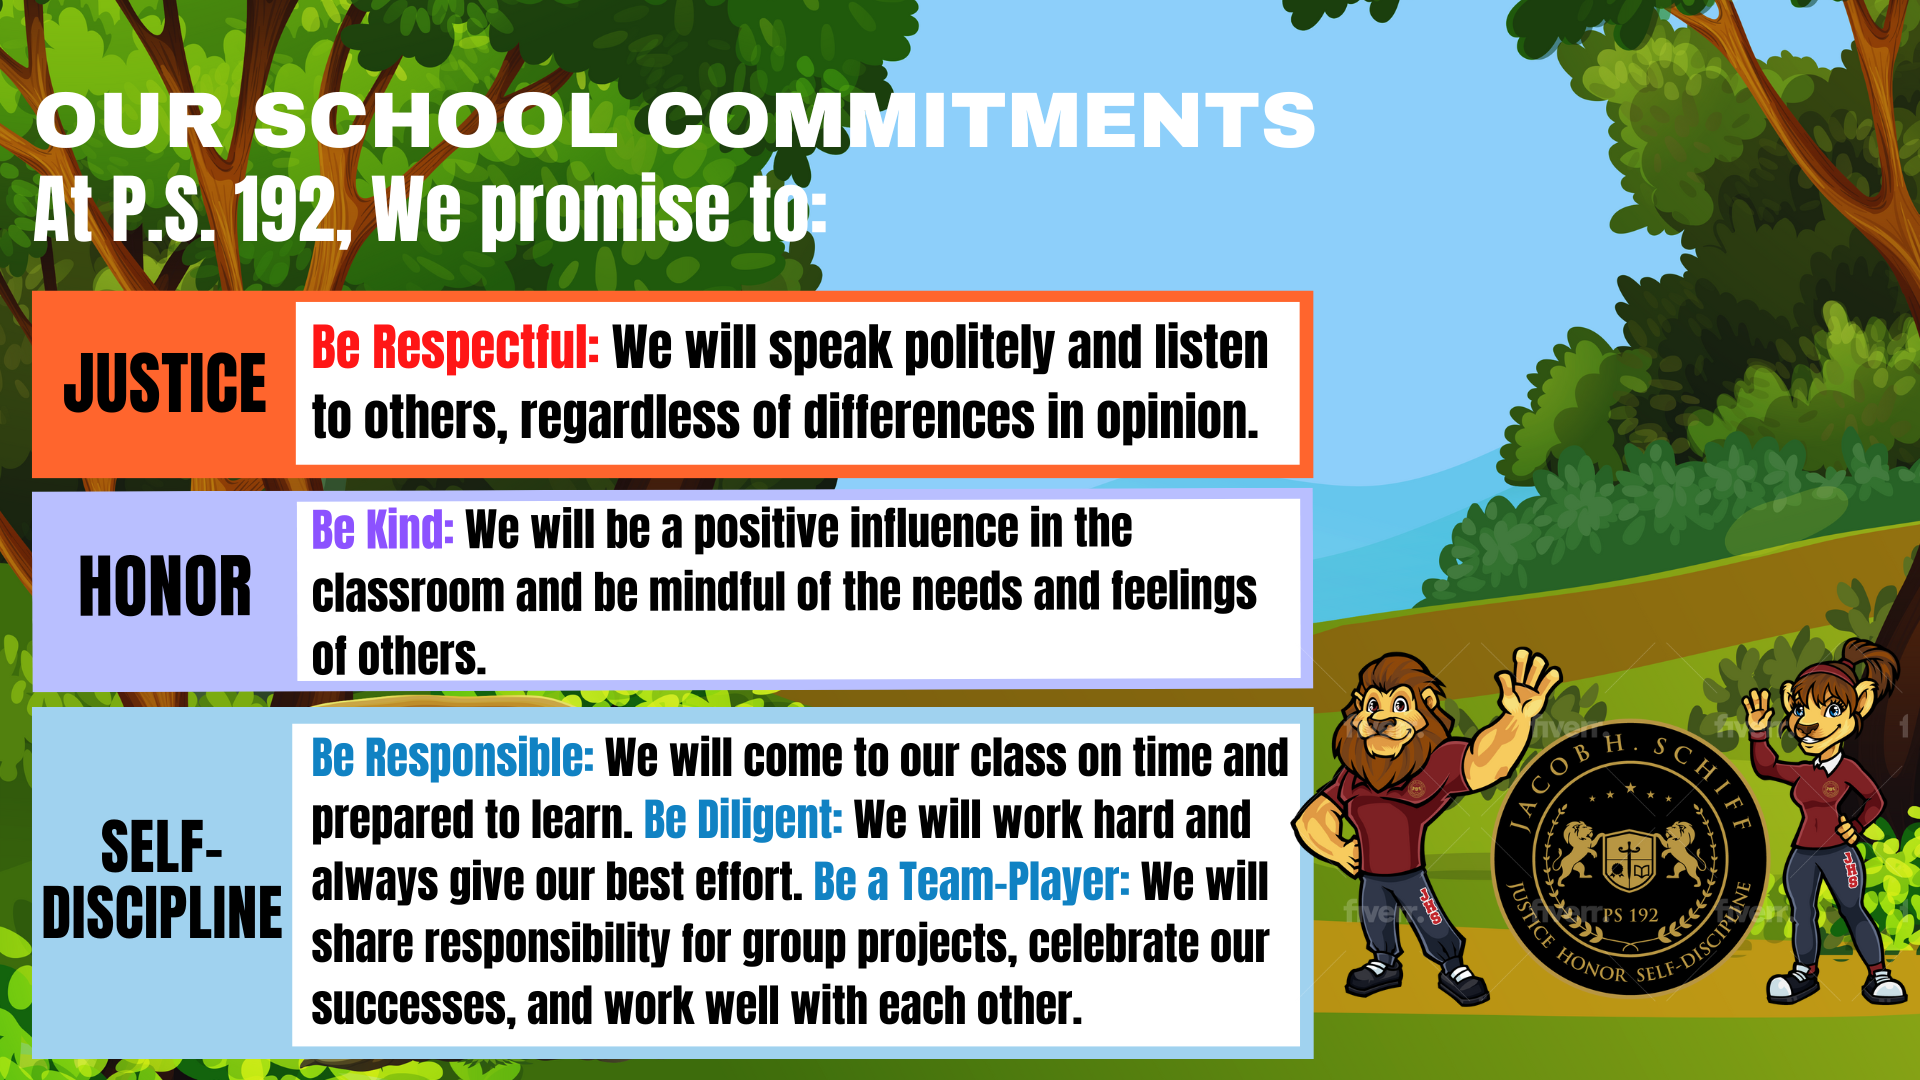
\includegraphics[width=0.9\textwidth]{commitments1}
  \caption{Students Commitments}
  \label{fig:Growth}
\end{figure}

\pagebreak
\end{document}
